%
% domain.tex -- domain for problem 90000019
%
% (c) 2019 Prof Dr Andreas Müller, Hochschule Rapperswil
%
\documentclass[tikz]{standalone}
\usepackage{amsmath}
\usepackage{times}
\usepackage{txfonts}
\usepackage{pgfplots}
\usepackage{csvsimple}
\usetikzlibrary{arrows,intersections,math}
\begin{document}
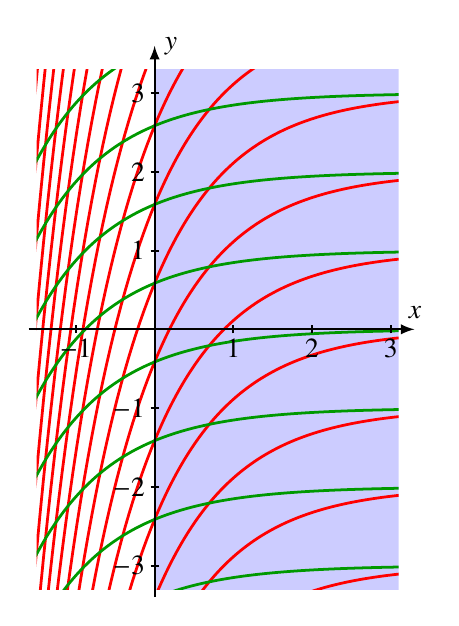
\begin{tikzpicture}[>=latex]

\definecolor{darkgreen}{rgb}{0,0.6,0}

\begin{scope}
\clip (-1.5,-3.3) rectangle (3.1,3.3);

\fill[color=blue!20] (0,-4)--(4,-4)--(4,4)--(0,4)--cycle;

\foreach \c in {-5,...,20}{
	\draw[color=red,line width=1pt]
		plot[domain=-1.55:3.1,samples=100] ({\x},{-(sqrt(2)+1)*exp(-\x)+\c});
}

\foreach \c in {-4,...,4}{
	\draw[color=darkgreen,line width=1pt]
		plot[domain=-1.55:3.1,samples=100] ({\x},{-(sqrt(2)-1)*exp(-\x)+\c});
}

\end{scope}

\foreach \x in {1,2,3}{
	\draw[line width=0.7pt] (\x,-0.05)--(\x,0.05);
	\node at (\x,0) [below] {$\x$};
}
\draw[line width=0.7pt] (-1,0.05)--(-1,-0.05);
\node at (-1,0) [below] {$-1$};

\foreach \y in {1,2,3}{
	\draw[line width=0.7pt] (-0.05,\y)--(0.05,\y);
	\draw[line width=0.7pt] (-0.05,-\y)--(0.05,-\y);
	\node at (0,\y) [left] {$\y$};
	\node at (0,{-\y}) [left] {$-\y$};
}

\draw[->,line width=0.7pt] (-1.6,0)--(3.3,0) coordinate[label={$x$}];
\draw[->,line width=0.7pt] (0,-3.4)--(0,3.6) coordinate[label={right:$y$}];

\end{tikzpicture}
\end{document}

